\begin{figure*}[t]
  \centering
  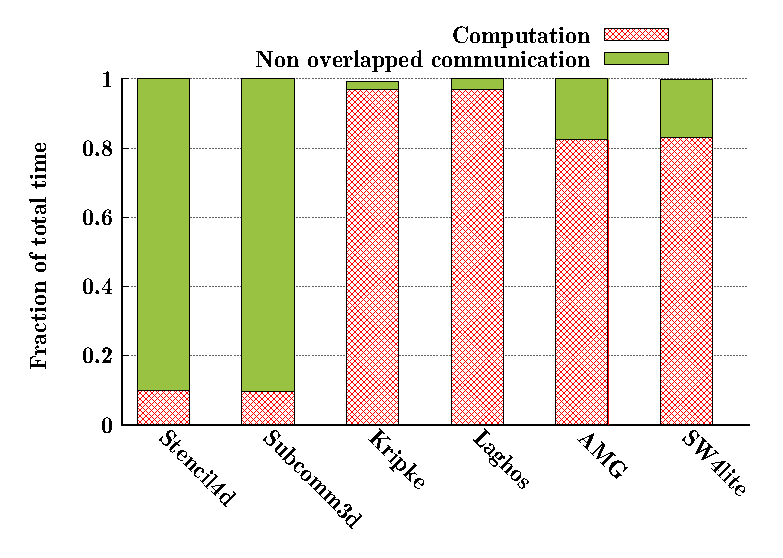
\includegraphics[width=0.8\columnwidth]{figure/val/mpi-scaled.eps}
  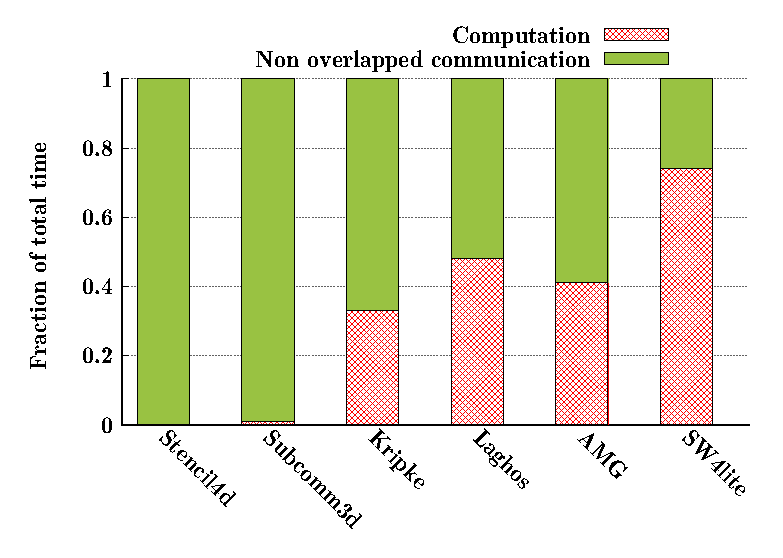
\includegraphics[width=0.8\columnwidth]{figure/val/mpi.eps}
  \caption{Computation and communication characteristics of all applications without scaling (left) and with scaling for GPUs (right)
running on 32 processes.} 
  \label{fig:trace_profile}
\end{figure*}


% The experiment has two components. First, I validate the TraceR-CODES
% framework by comparing simulation results with measurement results on a real
% supercomputer. Second, I study the impact of the hardware parameters on the
% performance. In the following, I will give details about our experiment
% design and configuration.

\label{sec:applicationworkload}

I selected six applications of different computation and communication
characteristics to create realistic HPC workloads. The applications include two
communication-heavy kernels, Stencil4d\cite{bhatele2018evaluating} and Subcomm3d\cite{bhatele2018evaluating}, two compute-intensive
applications, Kripke\cite{kripke} and Laghos\cite{laghos}, and two applications with a balanced
communication-to-computation ratio, AMG\cite{amg} and SW4lite\cite{sjogreen2018sw4} (see
Figure~\ref{fig:trace_profile}).  The traces used in the study were
collected using Score-P \cite{knupfer2012score} on Vulcan, a Blue Gene/Q
installation and Quartz, an Intel Xeon cluster at Lawrence Livermore National
Laboratory (LLNL). The traces contain information about all MPI events executed on each MPI process, along with their
timestamps. In addition, they also record user annotations such as loop
begin and end for the main compute loop. A brief description for the applications in provided in Chapter 2. 


\begin{comment}
Following
is a brief description of the six applications:

\begin{itemize}
\item \textbf{Stencil4d}: MPI benchmark with 8-point near-neighbor communication in a 4D virtual process grid.
\item \textbf{Subcomm3d}: MPI benchmark with all-to-all communication within subsets of processes in a 3D virtual process grid.
\item \textbf{Kripke}: 3D $S^n$ deterministic particle transport code, which runs an
  MPI-based parallel sweep algorithm.
\item \textbf{Laghos}: Proxy application that solves time-dependent Euler equations with MPI-based
  domain decomposition.
\item \textbf{AMG}:  Parallel algebraic multigrid solver.
\item \textbf{SW4lite}: Proxy application for SW4~\cite{sjogreen2018sw4}, a 3D seismic modeling code.
% The computational domain is discretized on one Cartesian mesh and optionally
% on one curvilinear mesh that follows a simple topography.
\end{itemize}
\end{comment}

Figure~\ref{fig:trace_profile} presents the fraction of total execution
time these applications spend in communication and computation when running
with 32 processes.  Computation is denoted by the red color, and non-overlapped
communication is shown in green. At 32 processes, Stencil4d and Subcomm3d are
dominated by communication. The communication-computation ratios were tuned in
Stencil4d and Subcomm3d such that they replicate the runtime profiles of
representative communication-intensive applications.  Kripke and Laghos are
dominated by computation with both spending more than 95\% of the time in computation.
AMG and SW4lite spend $\sim$80\% of their time in computation and the rest in
communication.  Suitable
computation scaling factors are used to alter the behavior of these traces to
emulate running the computation on GPUs. Figure~\ref{fig:trace_profile} 
shows how the computation-to-communication ratios change as these
scaling factors are applied. Stencil4d and Subcomm3d spend most of their time in
communication after compute scaling and the other applications now spend
between 25-65\% in communication.

The workloads in the study are created using the six HPC applications mentioned
above at different process counts -- 32, 64, 128, 256, and 512.  In this study,
the system supports up to 2048 processes. Thus, the sum of process counts in
each of the workloads is exactly 2048.  Each workload is obtained by
iteratively randomly selecting an application and a job size until the total
workload size has reached 2048.  As a result, each workload has many jobs of
different sizes, resembling the capacity workload of supercomputing
centers~\cite{jain2016evaluating}.  This study's experiments use 20 such random
workloads. To ensure that the reported performance of each job size of each
application is representative, each job size of each application
appears at least four times in the 20 workloads. This warrants that each job
size of each application has been executed under different conditions in the
experiments.
 
